\documentclass[a4paper,11pt]{article}

\usepackage[utf8]{inputenc}
\usepackage{graphicx}
\usepackage{minted}

\begin{document}

\title{
    \textbf{Mandelbrot}
}
\author{Malcolm Liljedahl}
\date{Spring Term 2022}

\maketitle

\section*{Introduction}
For this assignment we were supposed to create a Mandelbrot generator which works as an image generator.

\section{Step 1 - Complex numbers}
The first step was to create a module which handles some complex number calculations. A complex number both got an imaginary and a real part, so an obvious choice here would be to represent complex numbers as tuples.

\begin{minted}{elixir}
#creates a complex number
def new(r, i) do {r, i} end

#various calculations for the complex numbers
def add({a, ai}, {b, bi}) do {a+b, ai+bi} end

def sqr({r, i}) do {r*r - i*i, 2*r*i} end

def abs({r, i}) do :math.sqrt(r*r + i*i) end
\end{minted}


\section{Step 2 - Brot module}
The second step was to implement a module called Brot but I called it Mandelbrot due to some bugs with creating the mix project. It will implement a computation of the imaginary part i given a complex number c.

\begin{minted}{elixir}
#Implements the computation of i given the complex value c.
def mandelbrot(c = {r, i}, m) do # m = maximum iterations
    z0 = Cmplx.new(0, 0)
    i = 0
    test(i, z0, c, m)
end
\end{minted}
A test function was also created to test if we have reach our maximum amount of iterations. Even though the code might be better if I would have used case's here instead, I think that if/else did the job. 

\begin{minted}{elixir}
def test(m, z, c, m) do 0 end

def test(i, z, c, m) do
    var = Cmplx.abs(z)
    if var <= 2.0 do
      var2 = Cmplx.add(Cmplx.sqr(z), c)
      test(i+1, var2, c, m)
    else i
    end
end
\end{minted}

\section{Step 3 - Colors}
The next step was to create a module called Colors, which job is to give the image we generate more depth via colors. This module was simply created by following the guidelines of the assignment.

\begin{minted}{elixir}  
def convert(depth, max) do

    f = depth / max
    a = f * 4
    x = trunc(a)
    y = trunc(255 * (a - x))
    case x do
      0 ->
        {:rgb, y, 0, 0}
      1 ->
        {:rgb, 255, y, 0}
      2 ->
        {:rgb, 255 - y, 255, 0}
      3 ->
        {:rgb, 0, 255, y}
      4 ->
        {:rgb, 0, 255 - y, 255}
    end

end

\end{minted}

\section{Step 4 - Mandel}
Now it's time to calculate a whole image. And for that task the module Mandel was created. The following function were given to us and will work as our "interface".
To be able to generate the whole picture we use a function called rows, which should return a list of rows and each row is a list of colors.

\begin{minted}{elixir} 
def mandelbrot(width, height, x, y, k, depth) do
    trans = fn(w, h) ->
        Cmplx.new(x + k * (w - 1), y - k * (h - 1))
    end
    rows(width, height, trans, depth, [])
end
\end{minted}

\section{Conslusion}
With the code above this picture could be generated: 

\begin{figure}[H]
    \centering
    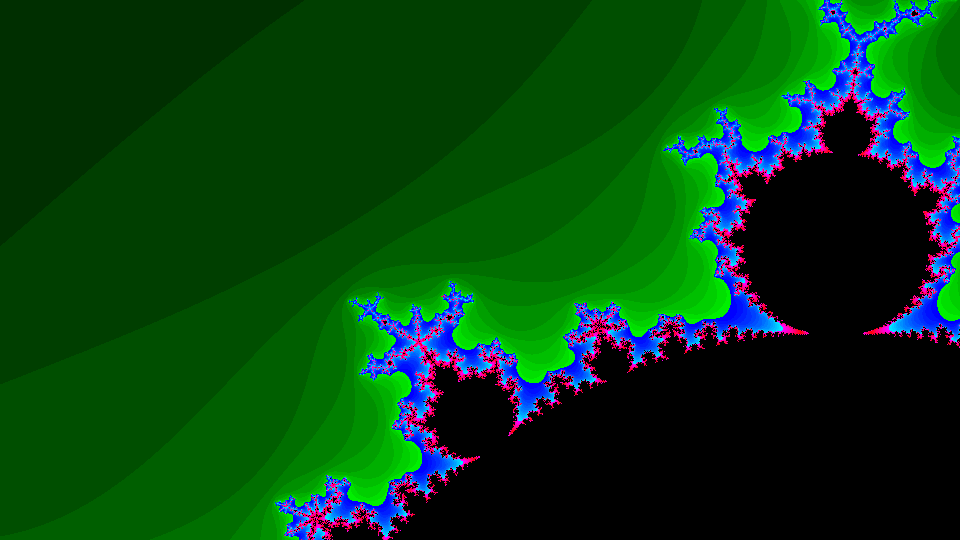
\includegraphics[scale=0.30]{small (19).png}
    \caption{Top view of the most zoomed out Mandelbrot set. Coordinates: (-0.9, 1.05, 0.005).}
\end{figure}


\end{document}